\section{Measurement uncertainties}
\label{sec:uncertainties}
An important aspect of an experimental measurement is characterizing its uncertainty. Broadly speaking, uncertainties can be divided into two types. The first is the statistical uncertainty, which is caused by inherently unpredictable fluctuations and can be reliably estimated by making repeated measurements~\cite{Kar:ab1be6}. The second is the category of systematic uncertainties, which arise in the estimation of systematic effects such as background, selection bias, scanning efficiency, energy resolution, angle resolution, variation of counter efficiency with beam position and energy, dead time, etc\cite{orear}. Systematic uncertainties are generally more difficult to determine, and cannot be calculated simply from sampling fluctuations \cite{reygers}. The total uncertainty of the measurement is the sum in quadrature of each individual component.

The breakdown and contribution of the uncertainty sources is shown in Figure \ref{fig:m4lsystematics} for the inclusive \mFourL{} spectrum. The dominant is the statistical uncertainty in all but the third mass bin with resonant single $Z$ production, where the lepton efficiencies' uncertainty prevails. Table \ref{tab:SysTablePerSlice} shows the breakdown of the uncertainties on the total fiducial unfolded cross-section, as well as the fiducial cross-section in the four \mFourL{} regions. The data statistical uncertainty plays a dominant role, followed by the uncertainty from the choice of generator. The rest of this section will discuss the different sources of uncertainty and how they are propagated.

\begin{figure}
    \centering
    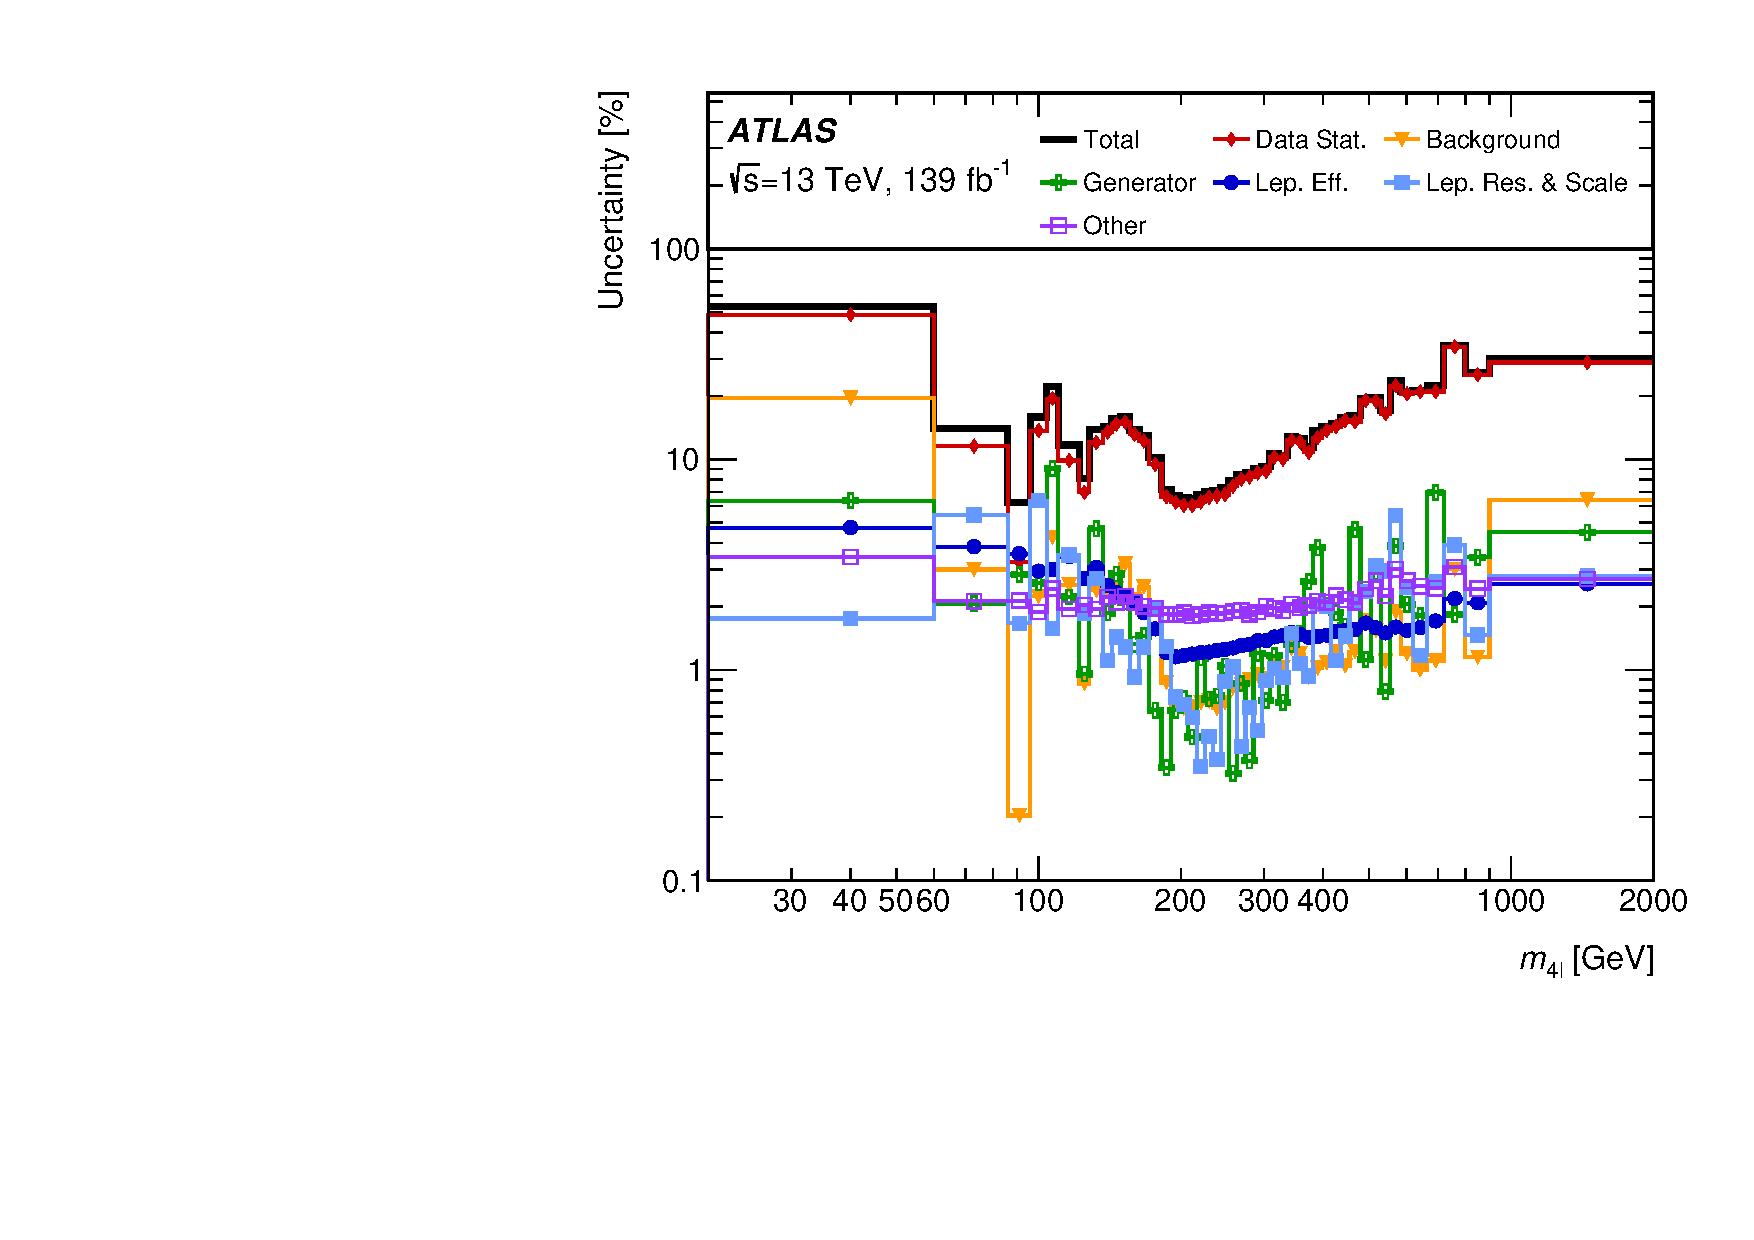
\includegraphics[width=0.85\textwidth]{Figures/m4l/Systematics/UnfoldedSys_M4l_Stack_Paper.pdf}
    \caption{Unfolded systematics for the inclusive \mFourL{} spectrum. The data statistical uncertainty is the dominant source in all but the third bin. This figure is from Ref.~\cite{m4l2021_paper}}
    \label{fig:m4lsystematics}
\end{figure}
\begin{table}
    \centering 
     \begin{tabular} {c  c  c  c  c  c }
         \hline 
         Region  & Inclusive   & $Z\rightarrow 4\ell$   & on-shell $H$   & off-shell $ZZ$   & on-shell $ZZ$   \\
         $m_{4\ell}$ [GeV]  & any   & 60-100   & 120-130   & 20-60/100-120   & 180-2000   \\
            &       &       &       & /130-180 & \\
         \hline 
        DD Closure &  $ 0.088\% $  &  $ 0.35\% $  &  $ 0.13\% $  &  $ 0.45\% $  &  $ 0.035\% $ \\
        Electron ID &  $ 0.94\% $  &  $ \mathbf{1.9}\% $  &  $ \mathbf{1.5}\% $  &  $ \mathbf{1.3}\% $  &  $ 0.49\% $ \\
        Electron Isolation &  $ 0.52\% $  &  $ \mathbf{1.1}\% $  &  $ 0.79\% $  &  $ 0.73\% $  &  $ 0.18\% $ \\
        Electron Reco &  $ 0.84\% $  &  $ \mathbf{1.7}\% $  &  $ \mathbf{1.3}\% $  &  $ \mathbf{1.2}\% $  &  $ 0.31\% $ \\
        Electron Res. \& Scale &  $ 0.46\% $  &  $ \mathbf{1.1}\% $  &  $ 0.83\% $  &  $ 0.54\% $  &  $ 0.12\% $ \\
        Generator &  $ \mathbf{1.3}\% $  &  $ \mathbf{2.6}\% $  &  $ \mathbf{1.3}\% $  &  $ \mathbf{2.7}\% $  &  $ 0.13\% $ \\
        MC Stat. &  $ 0.087\% $  &  $ 0.22\% $  &  $ 0.38\% $  &  $ 0.26\% $  &  $ 0.088\% $ \\
        Muon Isolation &  $ 0.96\% $  &  $ \mathbf{1.6}\% $  &  $ \mathbf{1.2}\% $  &  $ \mathbf{1.2}\% $  &  $ 0.58\% $ \\
        Muon Reco \& ID &  $ 0.83\% $  &  $ \mathbf{1.1}\% $  &  $ 0.91\% $  &  $ 0.89\% $  &  $ 0.82\% $ \\
        Muon Res. \& Scale &  $ 0.3\% $  &  $ 0.65\% $  &  $ 0.55\% $  &  $ 0.53\% $  &  $ 0.13\% $ \\
        Muon TTVA &  $ 0.21\% $  &  $ 0.46\% $  &  $ 0.28\% $  &  $ 0.31\% $  &  $ 0.071\% $ \\
        Non-Generator Theory &  $ 0.27\% $  &  $ 0.31\% $  &  $ 0.23\% $  &  $ 0.45\% $  &  $ 0.27\% $ \\
        Pile-up &  $ 0.73\% $  &  $ \mathbf{1.2}\% $  &  $ \mathbf{1}\% $  &  $ 0.81\% $  &  $ 0.47\% $ \\
        Reducible &  $ 0.8\% $  &  $ 0.55\% $  &  $ \mathbf{1.7}\% $  &  $ \mathbf{2.5}\% $  &  $ 0.74\% $ \\
        Trigger &  $ 0.33\% $  &  $ 0.8\% $  &  $ 0.44\% $  &  $ 0.44\% $  &  $ 0.084\% $ \\
        \hline 
        Total Systematic &  $ 2.6\% $  &  $ 4.8\% $  &  $ 3.7\% $  &  $ 4.6\% $  &  $ 1.5\% $ \\
        Luminosity &  $ \mathbf{1.7}\% $  &  $ \mathbf{1.6}\% $  &  $ \mathbf{1.6}\% $  &  $ \mathbf{1.6}\% $  &  $ \mathbf{1.7}\% $ \\
        Data Stat. &  $ \mathbf{1.3}\% $  &  $ \mathbf{2.9}\% $  &  $ \mathbf{6.2}\% $  &  $ \mathbf{4.1}\% $  &  $ \mathbf{1.5}\% $ \\
        \hline 
        Total &  $ 3.3\% $  &  $ 5.8\% $  &  $ 7.4\% $  &  $ 6.4\% $  &  $ 2.7\% $ \\
        \hline 
     \end{tabular}
    \caption{Uncertainties on the unfolded fiducial cross-section inclusively as well as in the four $\mFourL$ slices studied in this analysis, split by source. Uncertainty contribution larger than $1\%$ are marked in bold to guide the eye. This table is from Ref.~\cite{m4l_internalnote}. \label{tab:SysTablePerSlice} }
\end{table}

\subsection{Statistical uncertainties} \label{ssec:statuncert}

Predominantly, the statistical uncertainty is the dominant uncertainty in most bins of the measured differential and double differential cross-sections. The bootstrap method~\cite{ATLAS_Bootstrap_2021} is used to calculate the statistical uncertainty on the data, and the MC. It is first necessary to construct pseudo-data (also called toys). For each set of pseudo-data, a random value is drawn in each bin following a Poisson distribution where the expectation value is the observed event count that that bin. In total, 3500 pseudo-datasets are generated. Each of these are propagated through the unfolding procedure described in Section \ref{sec:unfolding}. The root mean square of the difference between the unfolded pseudo-data and the unfolded data is taken as the statistical uncertainty in each bin. The statistical uncertainties obtained in this way are equivalent to frequentist confidence intervals in the large-sample limit, while in the bins with few entries, the quoted bands are known to be up to 10\% narrower than a frequentist confidence interval.

The above method of estimating the statistical uncertainty is used as the quoted uncertainty in the measurements. When testing the observed cross-sections against the Standard Model, however, a secondary approach - where the expected number of events is used in place of the observed number of events - is preferred. That is, the 3500 pseudo-datasets follow a Poisson distribution with the mean equal to the predicted reconstruction-level SM event yield. This was motivated by studies in constraining SM effective field theory coefficients where the former approach resulted in unreliable limits. For more details see Section \ref{sec:interpretations}.

\subsection{Systematic uncertainties} \label{ssec:systematics}
Systematic uncertainties arise in nearly every step of the measurement. It is the result of measuring something, or estimating something that is not perfectly known because of certain limitations\cite{barlow2002systematic}. Systematic uncertainties are either experimental or theoretical in nature. The former is common to all analyses and pertains to to the ATLAS detector, while the latter relates to the simulation of physics processes as well as to analysis techniques. 

\subsubsection{Experimental sources}
The flat uncertainty on the integrated luminosity for the for the 2015-2018 datasets of 139 fb$^{-1}$ is $\pm 1.7\%$. The integrated luminosity and uncertainty for the whole Run 2 data-taking period is derived based on a calibration of the luminosity scale using $x-y$ beam-separation scans, following a methodology similar to that detailed in reference \cite{ATLAS-2019-Luminosity}, and using the LUCID-2 detector for the baseline luminosity measurements \cite{Avoni-LUCID-2}. While this uncertainty is not relevant in the unfolding, it applies when converting event counts into a cross-section result as well as during the interpretations.

There is an uncertainty associated with pile-up reweighting, which refers to the reweighting of the Monte Carlo samples in order to reproduce the distribution of the number of $pp$ collisions per bunch crossing ($\mu$) observed in the data \cite{ATLAS_XS_pp}. The uncertainty arises from the modelling of pileup events, including uncertainties in the pp inelastic cross-section. The resulting effects on the measured distributions of this analysis is small.

Lepton identification, reconstruction and isolation, and lepton energy/momentum resolution and scale efficiencies and their uncertainties are derived from data using large samples of $J/\psi\rightarrow\ell\ell$ and $Z\rightarrow\ell\ell$ decays. The uncertainties on the performance are derived following the method reported in reference \cite{ATLAS_muon_reco_2016} for muons and references \cite{ATLAS_electron_efficiency_2015-2017}, \cite{ATLAS_electron_efficiency_2015-2016} for electrons. Typical uncertainties on the identification efficiencies are in the range between 0.5\% to 1.0\% for muons and 1.0\% to 1.3\% for electrons. 

The uncertainty from the non-prompt lepton background estimate has a size-able effect in the low- and high-mass tails of the \mFourL{} distribution, reach up to 11\% and 6.5\% in the first and last bins respectively. The details of the uncertainty estimate on the Fake Factor method is detailed in Section \ref{ssec:fakeuncertainty}.

\subsubsection{Theoretical sources}
The choice of the generator used for the simulation of the \qqFourL{} process in constructing the response matrix for unfolding (see Section \ref{subsec:unfmethod}) is the largest source of theory-related systematic uncertainty. The uncertainty arises from the difference in the modelling of the final-state radiation of photons between the \SHERPA{} prediction and the \POWHEG{} + \pythia{} prediction. To assess the uncertainty, the \POWHEG{} + \pythia{} sample is reweighted to match the \SHERPA{} sample. This is done so no double counting of the unfolding method uncertainty occurs. The data is then unfolded via the standard procedure using the reweighted \POWHEG{} + \pythia{} input. The envelope of the observed ratio between this result and the nominal unfolded result is taken as the generator uncertainty. From the choice of unfolding method, the uncertainty is evaluated using the data-driven closure test detailed in Section \ref{subsec:unfmethod}. 

Other theoretical uncertainties have minimal effect on the unfolding, although their effect is larger on the particle-level predictions that the data is compared against. Generator choice aside, the dominant source is from the factorization and renormalization scale variations, with smaller contributions from PDF uncertainties, parton shower uncertainties, next-to-leading order $k-$factor reweighting uncertainties. Overall, this indicates that a good level of model-independence is achieved.

